\par A equação de Schrödinger mostra que átomos confinados possuem níveis de energia quantizados, conforme foi abordado anteriormente para o caso do elétron confinado em um potencial periódico. Num cristal, existem aproximadamente $10^{23}$ átomos por centímetro cúbico. Como os átomos em um material estão próximos um do outro, as funções de onda dos elétrons se superpõem, principalmente as dos elétrons da camada de valência. O princípio de exclusão de Pauli afirma que eles não podem ocupar os mesmos níveis de energia e, juntamente com a ação de um potencial, é criada uma distribuição de níveis, conhecida como banda de energia. As regiões energeticamente proibidas são chamadas de \textit{gaps} de energia\cite{qm_fis6}.

\subsubsection{Condutores, semicondutores e isolantes}

	\par As bandas de energia\cite{qm_fis6} são preenchidas de formas distintas para os diferentes tipos de materiais. O mapeamento das bandas de energia de ponto a ponto nas zonas de Brillouin gera as estruturas de banda.

	\par Denomina-se por banda de condução, a banda de energia que é ocupada por elétrons que possuem energia maior que o nível de Fermi, promovendo a condutividade no material. Já a banda de valência é ocupada por elétrons que estão mais afastados do núcleo que os demais, sendo menos energética que a banda de condução.

	\begin{figure}[H]
      \caption{Bandas de energia para diferentes tipo de material (Adaptado de \cite{bulk1})}
      \centering
      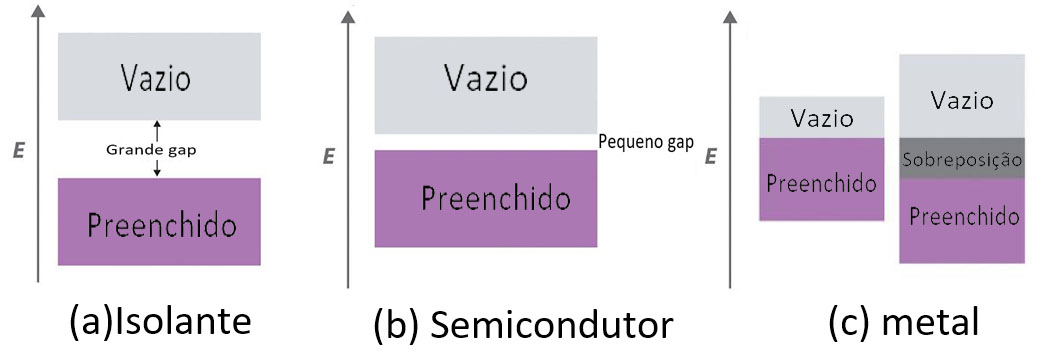
\includegraphics[width=0.75\textwidth]{images/figura3.jpg}
      \label{fig3}
    \end{figure}

	\par \textbf{- Metais}
	
		\par Para que o elétron possa conduzir num metal ele precisa possuir energia acima da energia de fermi, Ef. Nesse tipo de material existem estados livres adjacentes aos estados com a energia de fermi, já que existe superposição entre as bandas de valência e condução. Portanto, muito pouca energia é necessária para que se faça um elétron de um metal conduzir. A figura \ref{fig3}a ilustra as bandas de energia num metal. 

	\par \textbf{- Isolantes}

		\par No caso dos isolantes existe um grande gap de energia entre as bandas de valência e condução, sendo necessária muita energia para que um elétron conduza. A figura \ref{fig3}b ilustra as bandas de energia um isolante.

	\par \textbf{- Semicondutores}
	
		\par Finalmente, para os semicondutores, categoria à qual os pontos quânticos pertencem, existe, como nos isolantes, um gap de energia entre as bandas de valência e condução. Porém, o gap para esses materiais é menor do que nos isolantes. Sendo assim, é possível que alguns elétrons da camada de valência saltem para a de condução se alguma energia for fornecida ao semicondutor. Essa energia pode ser, por exemplo, térmica ou eletromagnética. A figura \ref{fig3}c ilustra as bandas de energia de um semicondutor.

\subsubsection{Semicondutores \textit{bulk}}

	\par Quando as dimensões dos materiais são reduzidas à nanoescala, propriedades interessantes aparecem. O impacto desse confinamento depende de cada material e da propriedade a ser analisada. Para a análise das propriedades ópticas de nanocristais semicondutores, por exemplo, leva-se em consideração o raio de Bohr, pois essa dimensão descreve espacialmente os éxcitons, que são pares elétron-buraco e serão retomados em tópicos posteriores. O confinamento espacial deles é conhecido como confinamento quântico. Para entender esse confinamento, é necessária uma abordagem da estrutura e das transições eletrônicas de semicondutores \textit{bulk}. 

	\par \textbf{- Estrutura Eletrônica de Semicondutores \textit{bulk}}

		\par Diferentemente do que ocorre para o elétron livre, um potencial periódico atua sobre o elétron em um semicondutor. Devido à periodicidade da rede e ao teorema de Bloch, sabe-se que a autofunção que satisfaz a propriedade de translação da rede é a função de onda de Bloch, definida anteriormente pela equação \eqref{bloch_3}.

		\par Novamente, para um elétron livre, a relação de dispersão é dada pela equação \eqref{schrodinger_3}, reescrita abaixo:

		\begin{equation}\label{eq_schrodinger_autovalores_rewrote}
	        E = \frac{\hbar^2 k^2}{2m}
	  	\end{equation}

	  	\par Essa relação pode ser observada na figura \ref{fig6}a

	  	\begin{figure}[H]
	      \caption{(a) Dispersão de energia para um elétron livre. (b) Dispersão de energia para um elétron perturbado por um potencial periódico. (c) Banda de energia para a primeira zona de Brillouin.}
	      \centering
	      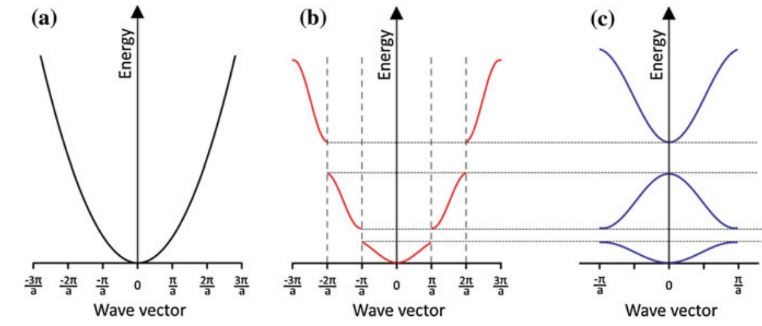
\includegraphics[width=0.75\textwidth]{images/figura6.jpg}
	      \label{fig6}
	    \end{figure}

	  	\par Ao perturbar a rede cristalina com um potencial periódico, ocorre uma mudança na relação de dispersão para o elétron. Essa perturbação provoca um gap de energia na região de degenerescência. Diz-se que um estado quântico é degenerado quando mais de uma função de onda está associada à mesma energia. Esse fenômeno pode ser observado na figura \ref{fig6}b. Os gaps de energia ocorrem para $\frac{n\pi}{a}$ porque os elétrons são refletidos, e essa reflexão é conhecida como reflexão de Bragg.

	  	\par A dispersão de energia pode ser restringida para valores de K entre $-\frac{\pi}{a} < K < \frac{\pi}{a}$, devido à periodicidade em K proporcionada pelo teorema de Bloch. Esse intervalo é conhecido como primeira zona de Brillouin. Quando a dispersão de energia é representada nela, tem-se a representação em zona reduzida. Considerando mais de um elétron nesse intervalo, configura-se a banda de energia, mostrada na figura \ref{fig6}c.

		\par Essa análise foi feita para o caso unidimensional. Para o caso tridimensional, a interpretação é mais complexa. Um exemplo desse último caso é mostrado na \ref{fig7}.

		\begin{figure}[H]
	      \caption{Estrutura de banda para o PbSe}
	      \centering
	      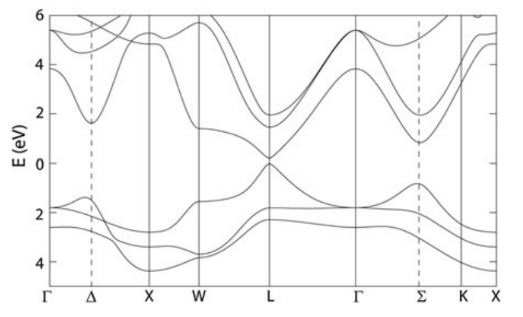
\includegraphics[width=0.75\textwidth]{images/figura7.jpg}
	      \label{fig7}
	    \end{figure}

		\par É válido ressaltar que  as estruturas de bandas podem ser calculadas por modelos teóricos, como o método k.p e o DFT (teoria do funcional de densidade).

		\par O método utilizado para o cálculo da estrutura de banda dos pontos quânticos é o \textit{one-band mass efective model}\cite{bulk2}. Como o  grau de dificuldade desses métodos é elevado, uma abordagem mais profunda foge do escopo neste trabalho.

	\par \textbf{- Transições eletrônicas para semicondutores bulk}

		\par Um semicondutor ideal na temperatura de zero Kelvin comporta-se como um isolante (estado fundamental). Ou seja, a banda de valência está totalmente preenchida e a banda de condução, vazia.
 		
 		\par Ao receber energia, alguns elétrons saltam para a banda de condução, fazendo com que buracos se desloquem para a banda de valência\cite{bloch1}. Buracos são orbitais vazios em uma banda de energia, que respondem a campos elétricos e magnéticos como se possuíssem carga +e\cite{qm_fis6}. O par elétron-buraco é chamado de éxciton e sua interação se dá pelo potencial de Coulomb\cite{bloch1}.

 		\par A energia mínima necessária para a formação do éxciton é dada por:

 		\begin{equation}
 			\label{bandas_1}
 			E = \hbar \omega = E_{g} + E_{e, kin} + E_{h, kin}
 		\end{equation}
 		onde $E_{g}$ representa o \textit{gap} de energia fundamental do semicondutor, $E_{e,kin}$ representa a energia cinética do elétron e $E_{h,kin}$, a energia cinética do buraco.

 		\par Da conservação de momento, tem-se:

 		\begin{equation}
 			\label{bandas_2}
 			\hbar \mathbf{k}_{cb} = \hbar \mathbf{k}_{vb} + \hbar \mathbf{k}_{foton}
 		\end{equation}

 		\par O termo $\mathbf{k}_{vb}$ é o vetor de onda para o elétron na banda de valência, $\mathbf{k}_{cb}$, o do buraco na banda de valência, e $\mathbf{k}_{foton}$, do fóton que tem momento despresível. Assim a relação $\mathbf{k}_{cb} = \mathbf{k}_{vb}$ deve ser satisfeita, como observado na figura \ref{fig8}

 		\begin{figure}[H]
	      \caption{Esquema de absorção de energia pelo elétron. Ao absorver o fóton, o elétron salta para a banda de condução.}
	      \centering
	      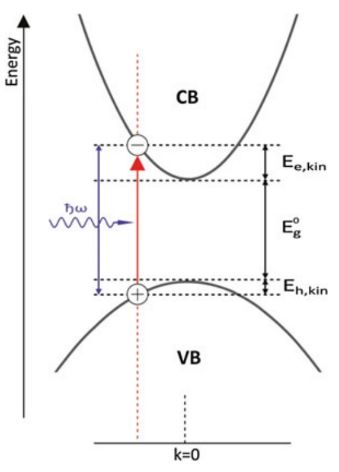
\includegraphics[width=0.35\textwidth]{images/figura8.jpg}
	      \label{fig8}
	    \end{figure}

\subsection{Heterojunções}

	\par Os pontos quânticos são formados por dois materiais semicondutores diferentes. A junção desses materiais constitui uma heteroestrutura, assim, é necessário entender como as estruturas de banda desses materiais se comportam na interface\cite{bulk2}.

	\begin{figure}[H]
	  \caption{Diagrama de energia de banda para uma heterojunção}
	  \centering
	  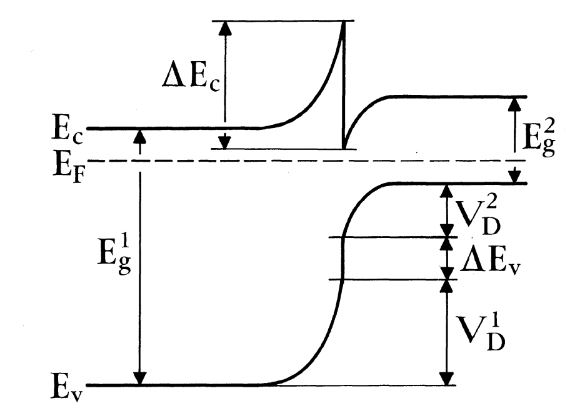
\includegraphics[width=0.5\textwidth]{images/figura14.jpg}
	  \label{fig14}
	\end{figure}

	\par A figura mostra dois tipos diferentes de semicondutores, com lacunas de energia $E_{g1}$ e $E_{g2}$. $E_{c}$ e $E_{v}$ se referem à borda da banda de condução e de valência, respectivamente. A energia de Fermi é denotada por $E_{f}$. $V_{d1}$ e $V_{d2}$ medem os dobramentos de bandas para os dois lados da heterojunção.

	\par A diferença de energia $E_{g1}-E_{g2}$ está associada a descontinuidades tanto na banda de valência quanto na banda de condução. Essas descontinuidades determinam as propriedades ópticas e de transporte para uma heterojunção e podem ser  visualizadas melhor na figura abaixo: 

	\begin{figure}[H]
	  \caption{Estrutura de banda para diferentes materiais}
	  \centering
	  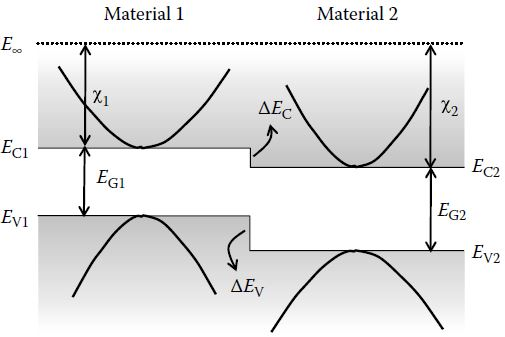
\includegraphics[width=0.5\textwidth]{images/figura15.jpg}
	  \label{fig15}
	\end{figure}

	\par Em 1962, R.R. Anderson publicou um artigo de referência sobre heterojunção baseado no modelo de Schottky para certos tipos de diodo REFERENCIAR HETEROJUNCAO. De acordo com o modelo de Anderson, as descontinuidades são obtidas por:

	\begin{equation}
		\label{bandas_3}
		\Delta E_{C} = \left|  \chi_{1} - \chi_{2} \right|
	\end{equation}

	\begin{equation}
		\label{bandas_4}
		\Delta E_{V} = \left| \left(E_{g1} + \chi_{1}\right) - \left(E_{g2} + \chi_{2}\right) \right|
	\end{equation}
	em que $\chi$ representa a afinidade eletrônica, que está relacionada com a energia necessária para retirar um elétron da banda de condução do material. 

	\par É relevante salientar que o modelo de Anderson só é válido para casos em que o desnível da rede é pequeno. 

	\par Elétrons e buracos podem estar confinados em um mesmo material ou em materiais diferentes, o que proporciona diferentes tipos de confinamento\cite{bulk2}.

